%%%% CAPÍTULO 2 - REVISÃO DA LITERATURA (OU REVISÃO BIBLIOGRÁFICA, ESTADO DA ARTE, ESTADO DO CONHECIMENTO)
%%
%% O autor deve registrar seu conhecimento sobre a literatura básica do assunto, discutindo e comentando a informação já publicada.
%% A revisão deve ser apresentada, preferencialmente, em ordem cronológica e por blocos de assunto, procurando mostrar a evolução do tema.
%% Título e rótulo de capítulo (rótulos não devem conter caracteres especiais, acentuados ou cedilha)
\chapter{revis\~ao Da Literatura}
\label{cap:revisaoDaLiteratura}

Esse capítulo apresenta os principais conceitos envolvidos na construção desse trabalho, a fim de contextualizar as bases teóricas utilizadas como referência para o desenvolvimento. O capítulo está organizado em duas seções, na primeira com aspectos do referencial teórico e na segunda com a apresentação de trabalhos relacionados.

\section{Computa\c{c}\~ao em Nuvem}
\label{sec:computacaoEmNuvem}

A computação em nuvem é um termo que se refere ao modelo de de entrega de recursos computacionais, baseado em uma grande rede de servidores físicos ou virtuais. Recursos como capacidade computacional ou capacidade de armazenamento são virtualizados em \textit{data centers} e consumidos sob demanda remotamente. Segundo \citet{taurioncloud}, as principais características são:

\begin{itemize}
    \item A computação em nuvem transmite uma sensação de disponibilidade infinita de recursos.

    \item Com esse tipo de modelo de serviços computacionais, não é necessário adquirir equipamentos físicos para poder utilizá-los. Os mesmo são acessáveis como serviços.

    \item Os recursos podem ser utilizados na proporção que são necessários para determinado cenário, podendo redimensionar a capacidade computacional de forma dinâmica.

    \item O modelo de cobrança em ambientes de nuvem é baseado na quantidade de uso dos recursos.
\end{itemize}

Os serviços de computação em nuvem podem ser classificados de acordo com o modelo de entrega de recursos, bem como o nível de responsabilidade que o usuário tem sobre a infraestrutura que suporta os serviços. Entre os modelos de entrega de recursos, os mais comuns são: \textit{Software as a Service} (SaaS), \textit{Platform as a Service} (PaaS) e \textit{Infrastructure as a Service} (IaaS). \citep{cloudcomputingcambridge}

A \autoref{fig:serviceDeliveryModels} apresenta um diagrama que ilustra a hierarquia de responsabilidades entre os modelos de entrega de recursos. O diagrama mostra que o \textit{SaaS} é o modelo que demanda menos responsabilidade do cliente, mas também entrega mais valor e abstração. O \textit{IaaS} é o modelo que demanda mais responsabilidade do cliente, mas também entrega mais controle sobre a infraestrutura. A \autoref{fig:deliveryModelResponsabilities} apresenta um diagrama que ilustra as responsabilidades de cada modelo de entrega de recursos. \citep{cloudcomputingcambridge}

\begin{figure}[H]
\captionsetup{width=.7\textwidth}%% Largura da legenda
\caption{Modelo de entrega de conteúdo em computação em nuvem}
\label{fig:serviceDeliveryModels}
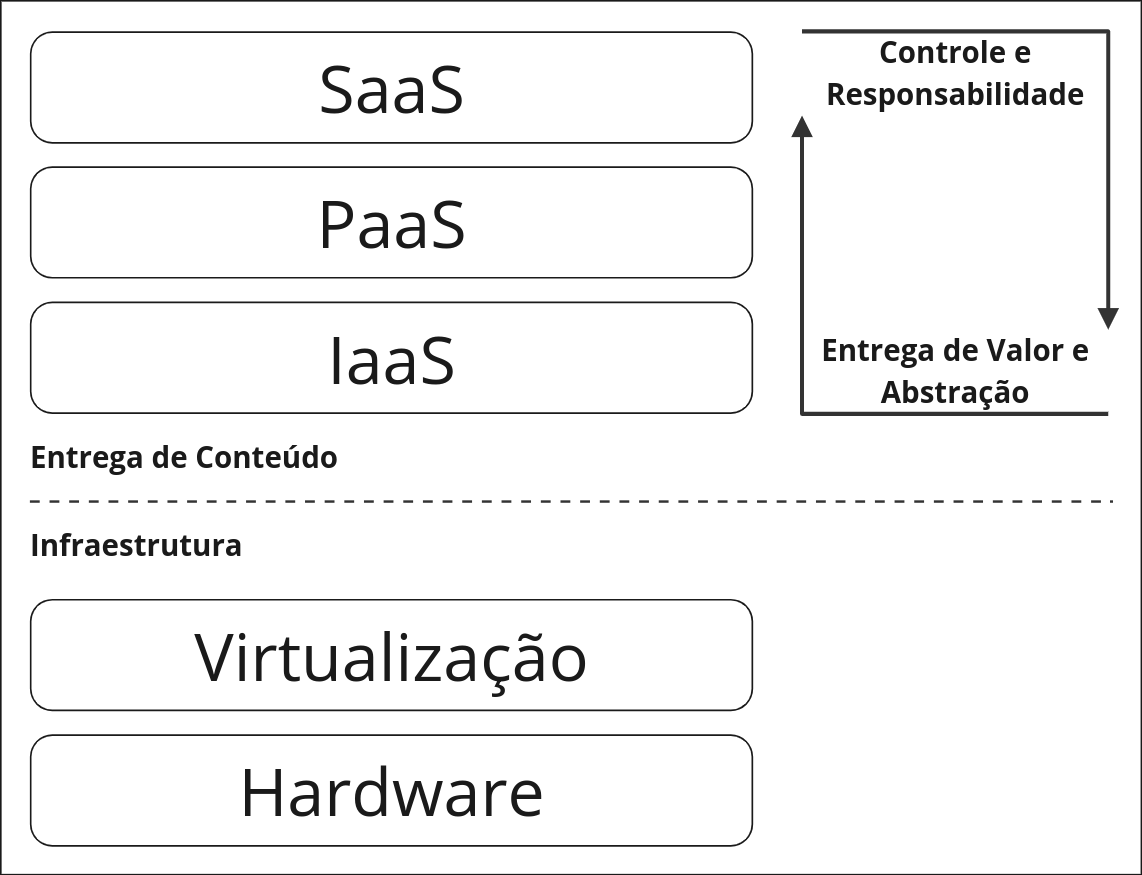
\includegraphics[width=.7\textwidth]{capitulos/1-revisao-da-literatura/files/deliovery-model.png}
\fonte{Adaptado de \citet{cloudcomputingcambridge}}
\end{figure}

\begin{figure}[H]
\captionsetup{width=.7\textwidth}%% Largura da legenda
\caption{Responsabilidades nos modelos de entrega de conteúdo em computação em nuvem}
\label{fig:deliveryModelResponsabilities}
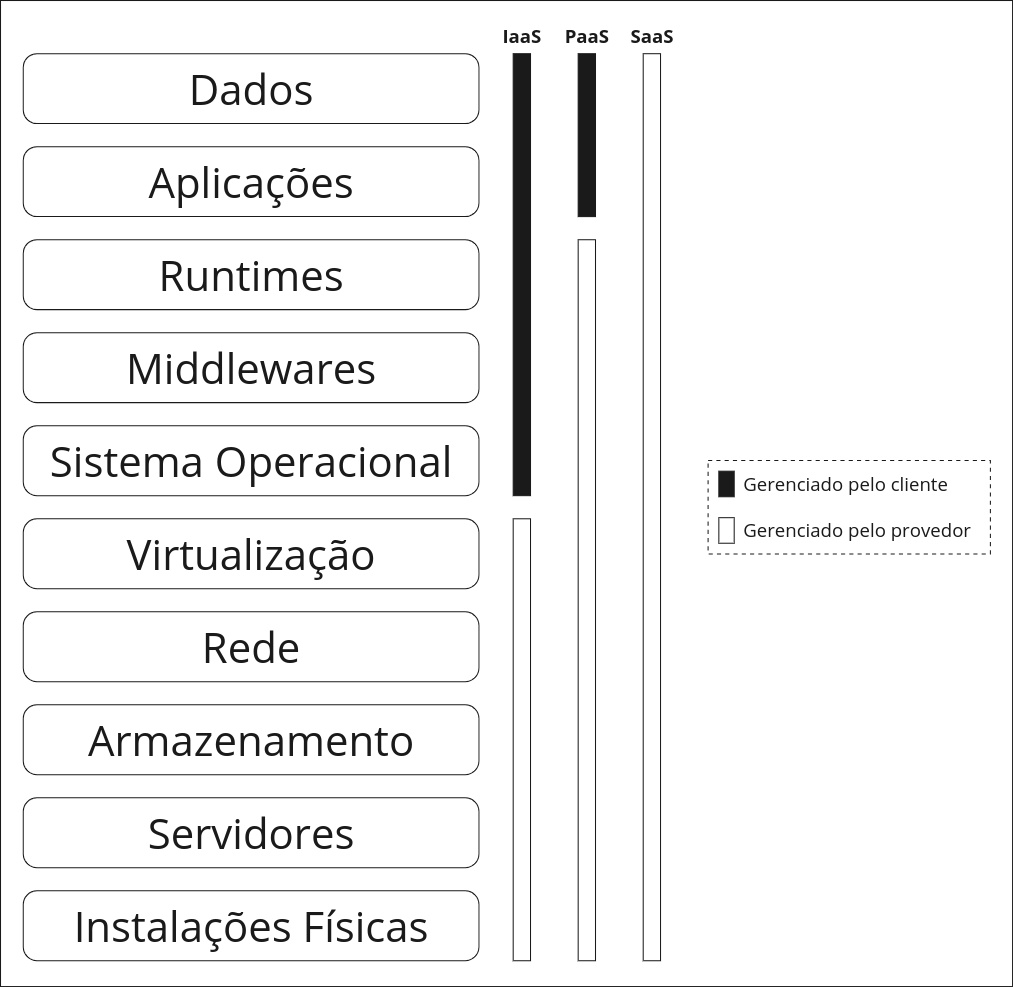
\includegraphics[width=.7\textwidth]{capitulos/1-revisao-da-literatura/files/delivery-model-2.png}
\fonte{Adaptado de \citet{cloudcomputingcambridge}}
\end{figure}

No modelo de entrega \textit{SaaS} o cliente acessa diretamente uma aplicação e o provedor é inteiramente responsável pelo gerenciamento e configuração da infraestrutura que o suporta. No \textit{PaaS} o cliente é capaz de executar e gerenciar aplicações sem a necessidade de se preocupar com a infraestrutura que suporta as aplicações e no \textit{IaaS} o cliente tem controle total sobre a todos os aspectos que compõem a representação virtualizada da infraestrutura. \citep{cloudcomputingcambridge}

Um exemplo de serviço gerenciável é o \textit{Elastic Beanstalk}, que é categorizado como \textit{Paas}. Com ele é possível executar aplicações sem a necessidade direta de configurar a maior parte dos serviços de infraestrutura disponíveis. O desenvolvedor precisa se preocupar somente com o código da aplicação.

Esse tipo de serviço é útil para soluções comuns como \textit{APIs} que necessitam na maioria dos casos dos mesmos componentes de infraestrutura como: Um servidor de aplicação, configuração de rede, balanceador de carga, banco de dados e um local para armazenamento de objetos.

A \textit{AWS} opera seus recursos a partir de um modelo de responsabilidade compartilhada que visa reduzir a responsabilidade operacional dos clientes sobre recursos. \citep{awssharedresponsibilitymodel} E seguindo o modelo, a sua responsabilidade é garantir a segurança \textbf{DA} nuvem. Isso significa que a provedora deve proteger todos os aspectos de infraestrutura que executa os serviços disponibilizados.

Para o cliente, a responsabilidade é de garantir a segurança \textbf{NA} nuvem, levando em consideração todas as boas praticas de desenvolvimento para que os recursos sejam utilizados de maneira responsável e segura.

\section{Virtualização}
\label{sec:virtualization}

A virtualização é uma técnica que permite a representação de recursos computacionais físicos através de uma camada de software que permite a utilização de recursos de maneira customizada e independente para cada necessidade, diferente da abordagem tradicional onde os recursos físicos são acessados diretamente. \citep{cloudcomputingcambridge}

Qualquer tipo de recurso computacional pode ser virtualizado, como processadores, memória, armazenamento e redes. Partindo de um modelo estrutural onde os recursos físicos são interligados e compartilhados, a virtualização permite a criação de ambientes isolados e independentes, onde cada recurso é acessado de maneira exclusiva. Ainda, a técnica de virtualização permite que um recurso físico seja representado através de múltiplos recursos virtuais, como mostra a \autoref{fig:virtualization}, viabilizando assim o modelo de Computação em Nuvem. \citep{cloudcomputingcambridge}

\begin{figure}[H]
\captionsetup{width=.7\textwidth}%% Largura da legenda
\caption{Transformação de recursos físicos em recursos virtuais através da virtualização}
\label{fig:virtualization}
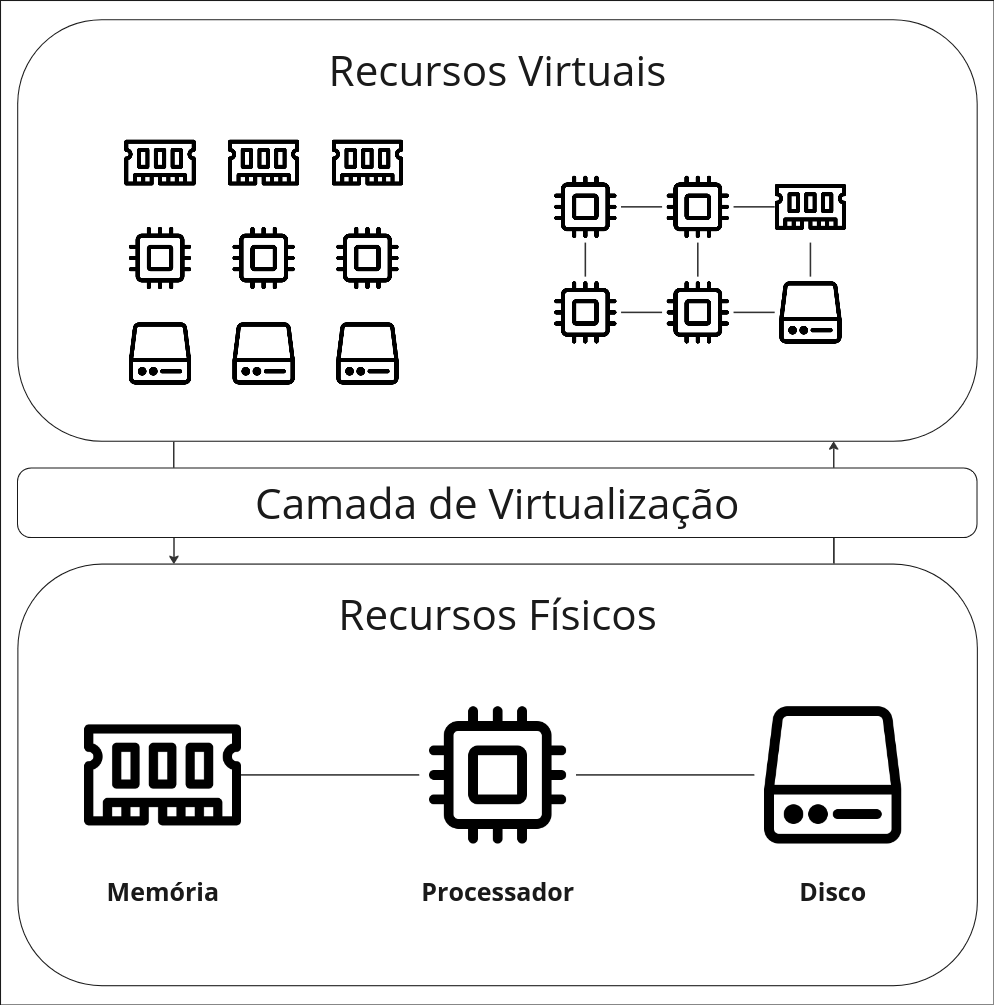
\includegraphics[width=.7\textwidth]{capitulos/1-revisao-da-literatura/files/virtualization-layers.png}
\fonte{Adaptado de \citet{cloudcomputingcambridge}}
\end{figure}

% Infraestrutura virtual de \textit{desktops} é uma técnica que permite o acesso a \textit{desktops} virtualizados através de uma conexão de rede. O conceito engloba os aspectos de hardware, software e infraestrutura necessários para o acesso remoto. \citep{techopediavdi}

% Em um ambiente de \textit{VDI}, todas as configurações de sistema operacional e preferências ficam armazenadas no \textit{host}. Para o usuário, a experiência de acesso é similar ao uso de um computador local.

% A maneira que os \textit{desktops}  são distribuídos entre os usuários depende da implementação do serviço e costuma seguir um dos dois padrões a seguir: \citep{vdiieexplore}

% \begin{enumerate}
%     \item Implementação dedicada: Nela, o \textit{desktop} é alocado especificamente para um usuário, e caso o ambiente não seja volátil, não é necessário a existência de um mecanismo de backup para as configurações salvas.

%     \item Implementação em pool: Nesse padrão, quando o usuário acessa um \textit{desktop}, o servidor cria a conexão com o próxima instância disponível no sistema. Isso significa que a cada acesso, as configurações serão reiniciadas para o padrão de inicialização do sistema. É comum nesses casos que o servidor mantenha um número mínimo de instâncias previamente inicializadas para diminuir o tempo de conexão.
% \end{enumerate}



% Arquitetura hexagonal
\section{Arquitetura Hexagonal}
\label{sec:arquiteturaHexagonal}

Arquitetura hexagonal é um padrão de arquitetura de software proposto por Alistair Cockburn em 2005, que ajuda a solucionar problemas de testabilidade e acoplamento de componentes em sistemas de software. Quando um software é projetado, muitas vezes é difícil projetar componentes genéricos o suficiente para que não dependam de um determinado \textit{framework} ou tecnologia. Isso é problemático porque a manutenção do software se torna mais difícil e a escolha de novas tecnologias pode ser limitada, além de tornar o processo de testes complexo e custoso. Para resolver esses problemas, a arquitetura hexagonal propõe uma abordagem onde o núcleo da aplicação é responsável por orquestrar todas as operações de entrada e saída de dados através de adaptadores. \citep{cockburn2017}.

Como pode ser visto na \autoref{fig:hexagonalArchitecture}, o padrão é representado por um hexágono com a aplicação no centro. As arestas do hexágono delimitam as fronteiras dos casos de uso da aplicação e também representam os \textit{Ports}, que são as interfaces as interfaces de comunicação entre a camada de aplicação e a camada de interfaces \citep{cockburn2017}.

\begin{figure}[H]
% \captionsetup{width=.7\textwidth}%% Largura da legenda
\caption{Arquitetura hexagonal}
\label{fig:hexagonalArchitecture}
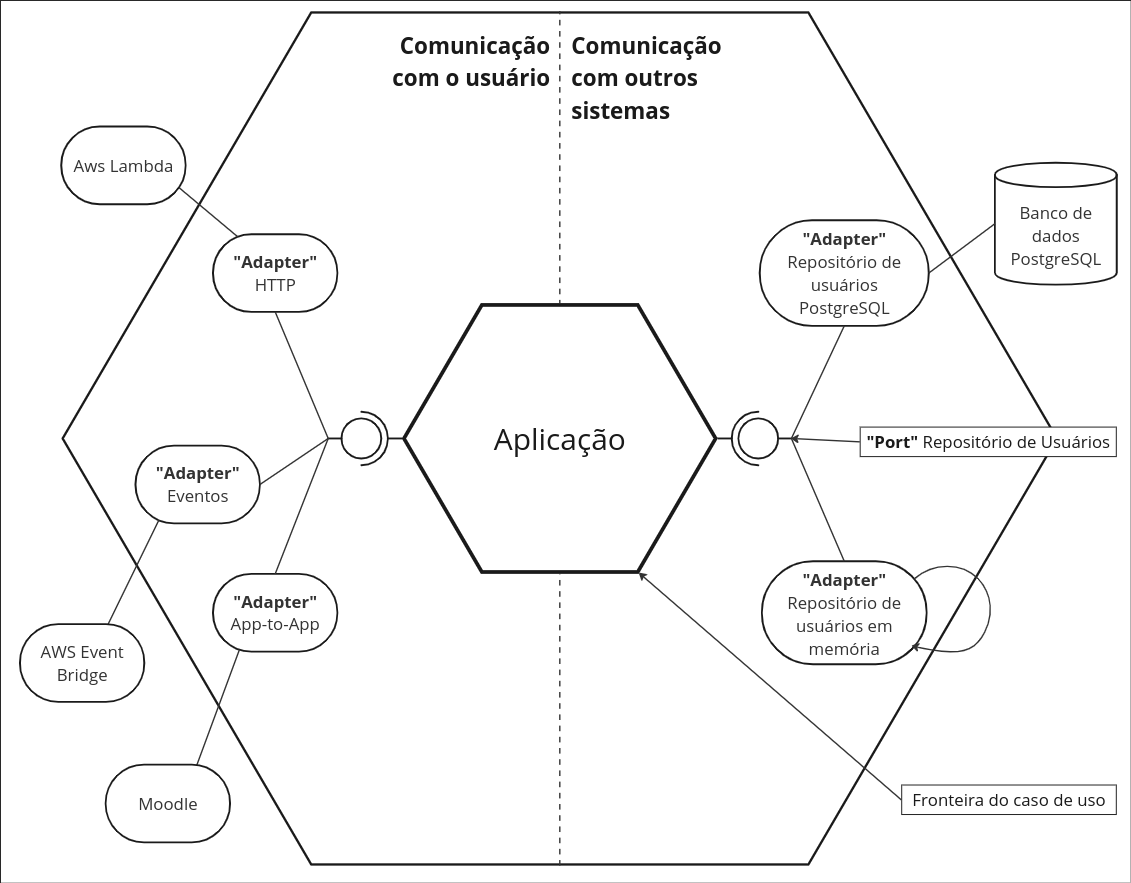
\includegraphics[width=\textwidth]{capitulos/1-revisao-da-literatura/files/hexagonal.png}
\fonte{Adaptado de \citet{cockburn2017} e \citet{awsHexagonalArchitecture}}
\end{figure}

Os adapter são classes que implementam as interfaces definidas pelos \textit{Ports}, neles a lógica de comunicação com quaisquer componente externo é implementada. Dessa forma, a aplicação não precisa saber de detalhes técnicos de cada componente externo, como por exemplo, a forma de comunicação com um banco de dados ou a forma de comunicação com um serviço de mensageria. \citep{cockburn2017}.

No momento da criação de testes unitários para os casos de uso da aplicação, os \textit{Adapters} que utilizam comunicação externa são substituidos por outros \textit{Adapters} que simulam a comunicação externa. Isso permite que os testes sejam executados de maneira independente e sem a necessidade de outros serviços externos. Na imagem \autoref{fig:hexagonalArchitecture}, existe um exemplo de \textit{Port} para armazenamento de informações de usuários, bem como dois \textit{Adapters} que implementam a interface do \textit{Port}. Um dos \textit{Adapters} é responsável por armazenar as informações em um banco de dados e o outro é responsável por armazenar as informações em memória. Ambos são utilizados dentro do ciclo de desenvolvimento, mas em momentos diferentes, sendo um para testes e outro para a execução real da aplicação.

No desenvolvimento prático utilizando \textit{Ports and Adapters}, padrões como o \textit{Domain Driven Design} o \textit{SOLID} e a injeção de dependências são comumente utilizados em conjunto \citep{cockburn2017}.





% A arquitetura hexagonal é um padrão de arquitetura de software proposto por Alistair Cockburn em 2005, com o objetivos de criar \textit{softwares} desacoplados onde os componentes possam ser testados de maneira independente. Além disso, o padrão ajuda a evitar que a implementação das regras de negócio fiquem acopladas a um determinado \textit{framework} ou tecnologia. \citep{awsHexagonalArchitecture}.


% Nesse padrão, a aplicação é representada por um exágono, onde cada lado representa uma porta de entrada ou saída de dados. As portas de entrada são responsáveis por receber os dados de entrada e as portas de saída são responsáveis por enviar os dados de saída. O núcleo da aplicação é responsável por orquestrar a comunicação entre as portas de entrada e saída. \citep{awsHexagonalArchitecture}.



\section{Trabalhos Relacionados}
\label{sec:trabalhosRelacionados}

O trabalho desenvolvido por \citet{qoselearning} realiza uma análise quantitativa do impacto de
parâmetros de conexão de rede em ambientes de ensino remoto sustentados por uma estrutura de \gls{vdi}.
A análise é feita a partir de um experimento com o objetivo de clarificar a relação entre a qualidade de
conexão com a internet e a usabilidade de sistemas de ensino remoto.

O resultado do experimento mostrou que é possível realizar atividades como escrita, desenhos e
consumo de mídias, sem grandes prejuízos para a usabilidade, mas é necessário que a conexão com a
internet tenha qualidade. Outro ponto importante é que fora atividades de visualização de vídeos, a
largura de banda não é um fator de grande consumo nesses tipos de ambientes.

Outro trabalho de grande relevância para essa produção, desenvolvido por \citet{edufirestick},
apresenta um sistema de \gls{vdi} para educação remota utilizando as mesmas tecnologias propostas
no presente trabalho. 

A proposta da produção é de criar uma \gls{vdi} de baixo custo com \glspl{ec2SpotInstance} da
\gls{aws} e com o \gls{guacamole} para gerenciamento das conexões, e permitindo o acesso de
qualquer dispositivo com um navegador de internet, até mesmo através televisões com acesso à internet,
como apresentado no trabalho.

A solução proposta por \citet{edufirestick} aborda um cenário de aula de laboratório, onde um
professor pode agendar um evento de criação das máquinas virtuais para os alunos e no horário da
aula, todos poderiam acessar o recurso reservado para a aula.

Em termos de custos operacionais, o trabalho apresenta uma estimativa de custo por usuário de
USD\$ 0.87 mensais com a utilização dos seguintes parâmetros:

\begin{itemize}
    \item Tempo de conexão diária: 18 horas
    \item Categoria da instância: t3.micro
    \item Sistema operacional: \textit{Microsoft Windows Server 2019}
    \item Memória: 4 GB de \gls{ram}
    \item Espaço em disco: 90 GB
    \item Região: São Paulo
\end{itemize}

Em termos de preço pela transferência de dados, o trabalho relata um custo de USD\$ 0.06 por hora em
picos onde o uso de banda chaga a 2 MB/s. O custo dos outros serviços que suportam a infraestrutura,
foi estimado em USD\$ 200.00 mensais.

O trabalho feito por \citet{edufirestick} apresenta um panorama muito promissor e consoante aos
objetivos do presente trabalho, demostrando que é possível executar a solução em um cenário de
laboratório. Mas ainda não apresenta resultados referentes ao gerenciamento de \glspl{desktop} que
tenham os dados persistidos, para outros cenários de uso, como o de pesquisa por exemplo.